\chapter{Documentación en GitHub: NYC-Taxi-Tip-Predictor} \label{chap:ap_b}

\vspace*{5mm}

\section{Introducción} \label{sec:b.1}

El código usado para poder escribir el capítulo \ref{chap:5} está disponible en forma de \emph{notebooks} de IPython, creados utilizando BMO, la herramienta presentada en el capítulo \ref{chap:4}. Además, este código esta disponible en GitHub, siendo este \emph{open source} bajo la \emph{licencia MIT}:

\url{https://github.com/josemazo/nyc-taxi-tip-predictor}

A continuación, en la seccción \emph{\ref{sec:b.2} \nameref{sec:b.2}}, se muestra una breve documentación del repositorio, donde además se ofrece un enlace a \emph{nbviewer}, una herramienta para poder visualizar notebooks de IPython online.

\section{README} \label{sec:b.2}

First of all, I must say thank you to \href{https://twitter.com/chris_whong}{Chris Whong} for obtaining the incredible dataset that it's used in this project. \href{http://chriswhong.com/open-data/foil_nyc_taxi/}{Here}\footnote{\url{http://chriswhong.com/open-data/foil_nyc_taxi/}} is his little odyssey to get the data.

\begin{figure}[H]
  \centering
  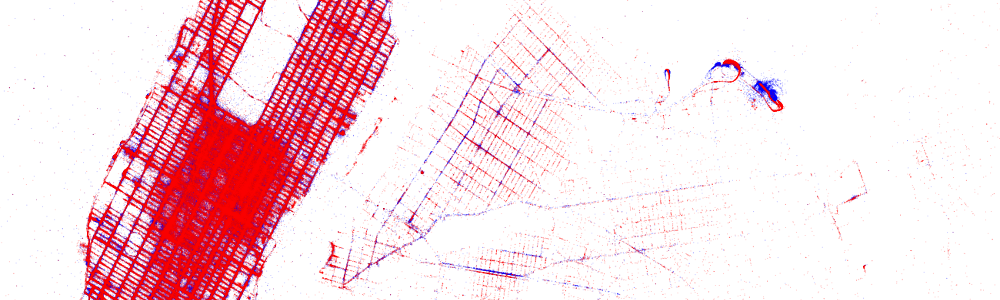
\includegraphics[width=140mm]{figures/ap_b/map.png}
  \label{fig:b.1}
\end{figure}

\Large
\textbf{TL;DR}

\normalsize
After cleaning and getting a sample from the original dataset, it's possible to predict, with an \emph{accuracy of 71.74\%}, if the tip of a trip in a NYC taxi it's going to be \emph{less thant 20\%} or \emph{greater than or equal to 20\%} of the charge.

\Large
\textbf{Extended version}

\normalsize
For read an extended version there are some IPython \emph{notebooks} that describe the complete process. You can find them in this repo, but for a better reading use \href{http://nbviewer.ipython.org/github/josemazo/nyc-taxi-tip-predictor/tree/master/notebooks/}{this \emph{nbviewer} link}\footnote{\url{http://nbviewer.ipython.org/github/josemazo/nyc-taxi-tip-predictor/tree/master/notebooks/}}.
